\documentclass[conference]{IEEEtran}
\IEEEoverridecommandlockouts
\usepackage{cite}
\usepackage{amsmath,amssymb,amsfonts}
\usepackage{algorithmic}
\usepackage{graphicx}
\usepackage{textcomp}
\usepackage{xcolor}
\usepackage{listings}
\usepackage{hyperref}

\def\BibTeX{{\rm B\kern-.05em{\sc i\kern-.025em b}\kern-.08em
    T\kern-.1667em\lower.7ex\hbox{E}\kern-.125emX}}

\lstset{
    language=Python,
    basicstyle=\ttfamily\scriptsize,
    keywordstyle=\color{blue}\bfseries,
    stringstyle=\color{red},
    commentstyle=\color{green!50!black},
    breaklines=true,
    captionpos=b,
    numbers=left,
    numberstyle=\tiny\color{gray},
    stepnumber=1,
    numbersep=5pt,
    tabsize=2,
    showstringspaces=false
}

\begin{document}

\title{AWD-COORD: Autonomous Multi-Node Alternate Wetting and Drying Irrigation Coordinator\\
}

\author{
\IEEEauthorblockN{
Mostafizur Rahman, Fahad Parvez Sagor, Saikat Raihan, \\
M. M. Sayem Prodhan, Sadid Ahmed, and Md. Mehedi Hasan
}
\vspace{1.5mm}
\IEEEauthorblockA{
\textit{Department of Computer Science \& Engineering} \\
\textit{United International University}\\
Dhaka, Bangladesh \\
\vspace{1.5mm}
Email: \{mrahman2330844, fsagor2330829, sraihan223611\}@bscse.uiu.ac.bd, \\
\{mprodhan2330411, sahmed2330154\}@bscse.uiu.ac.bd, mehedi@cse.uiu.ac.bd
}
}

\maketitle

\begin{abstract}
Traditional rice farming relies on continuous flooding, which uses excessive freshwater and depletes groundwater. Alternate Wetting and Drying (AWD) saves 25--50\% of water and reduces methane emissions, but applying it manually requires constant labor and causes conflicts when farmers share one pump. We present AWD-COORD, an IoT water management system that automates AWD and schedules pump access among multiple fields. It uses an ESP-NOW wireless mesh network for field sensors, a Python priority scheduler, a shadow failover node, and a cloud telemetry dashboard. We show that AWD-COORD resolves conflicts over shared pumps, manages hardware safely through power monitoring and actuation latencies, and sends plot-specific SMS alerts.
\end{abstract}

\begin{IEEEkeywords}
IoT, Alternate Wetting and Drying, Smart Agriculture, ESP-NOW, Resource Scheduling, Telemetry, ESP32
\end{IEEEkeywords}

\section{Introduction}

\subsection{Background}
Agriculture consumes more freshwater than any other global industry, and rice cultivation accounts for a large share of that use. Farmers traditionally grow rice in continuously flooded paddies. Flooding controls weeds, but it also depletes groundwater and creates anaerobic soil conditions that release high methane (CH$_4$) emissions. To reduce this, the International Rice Research Institute (IRRI) advocates for Alternate Wetting and Drying (AWD). This practice allows fields to dry to a specific threshold (typically 15 cm below the surface) before re-flooding. AWD saves 25--50\% of irrigation water and reduces greenhouse gas emissions without hurting crop yields.

\subsection{Motivation and Problem Statement}
Two factors limit the adoption of AWD: labor and shared infrastructure. Traditional AWD requires farmers to constantly check PVC perforated pipes in the mud to measure the underground water table. This manual labor is unmanageable at scale. In developing nations, smallholder farmers rarely own dedicated irrigation infrastructure; instead, they share one centralized diesel or electric pump. If multiple farmers practicing AWD need water at the same time, the conflicts lead to pump-hogging, dry crops, and social disputes. 

\subsection{Contributions}
To solve these problems, we built AWD-COORD, an IoT system that automates AWD and enforces fair pump access. Our primary contributions are:
\begin{itemize}
    \item \textbf{Automated AWD Agronomy:} An ESP-NOW wireless sensor network that monitors soil moisture, water depth, and crop growth stages to enforce AWD thresholds automatically (e.g., maintaining 5 cm depth during flowering).
    \item \textbf{Equity Priority Scheduling:} A centralized Python algorithm that calculates a priority score based on depth deficits, waiting time, and a historical equity penalty, so multiple farmers can share one pump without conflict.
    \item \textbf{Industrial-Grade Fault Tolerance:} Mechanical safety latencies to prevent pipe bursts and pump dry-runs, alongside a decoupled shadow node that executes an emergency shutdown if the master server crashes.
    \item \textbf{Multi-Tenant Telemetry and Alerting:} A SIM800L SMS routing system that alerts individual farmers to plot-level events, paired with a Google Sheets cloud telemetry dashboard.
\end{itemize}

\section{Related Work}
Alternate Wetting and Drying (AWD) reduces water usage by up to 30\% and lowers methane (CH$_4$) emissions \cite{lampayan2015}. However, its reliance on manual measurements inside PVC tubes makes it difficult to adopt at scale \cite{irri_awd}.

Researchers have used ultrasonic sensors and microcontrollers (e.g., Arduino, ESP32) to monitor water tables and automate pump activation \cite{iot_awd_ieee}. Low-power long-range networks such as LoRa and local mesh networks like ESP-NOW can relay this sensor data from fields to central dashboards \cite{espnow_wsn}.

Existing systems are generally designed for single-owner plots with dedicated pumps. Because multiple farmers share a single centralized pump in rural regions, the literature needs arbitration algorithms to prevent pump hogging. Many proposed systems also overlook hardware safety latencies (e.g., preventing pump dry runs or backpressure from slow valves) and lack fail-safe architectures for controller crashes \cite{safety_iot}. AWD-COORD addresses these gaps through multi-tenant equity scheduling and a localized failover mechanism.

\section{System Architecture and Network Design}
The AWD-COORD system uses embedded edge nodes, a backend control daemon, and a web dashboard for telemetry. The decoupled architecture improves reliability.

\subsection{Wireless Edge Network (ESP-NOW)}
Traditional Wi-Fi networks require a centralized router, making them impractical in agricultural fields. The system instead uses ESP-NOW, a connectionless peer-to-peer MAC-layer protocol on ESP32 microcontrollers, to form a low-latency mesh network. 
The network consists of four primary node types:
\begin{itemize}
    \item \textbf{Field Nodes:} Positioned in the rice plots to collect water depth, crop stage, and soil moisture. Each node broadcasts status payloads (\texttt{PKT\_FIELD\_STATUS}) every 1000 ms and heartbeat payloads (\texttt{PKT\_HEARTBEAT}) every 2000 ms.
    \item \textbf{Pump Node:} Controls the main 12V water pump using an L298N motor driver and monitors electrical power using an INA219 sensor. It also aggregates system-wide rain data.
    \item \textbf{Coordinator Proxy:} Acts as the gateway bridging the wireless ESP-NOW data to the wired USB serial bus of the master control machine.
    \item \textbf{Shadow Coordinator:} An independent ESP32 that solely listens for the Proxy's heartbeat. If the Proxy fails, the Shadow assumes control within 3 seconds to execute emergency hardware shutdowns.
\end{itemize}

\subsection{Python Backend Coordinator}
The python daemon runs on a master PC or Raspberry Pi to act as the system brain. It receives raw telemetry from the proxy over serial (baud 115200), parses it, and feeds it into a priority scheduling state machine. This Python layer handles the scheduling math, which is too heavy for the C++ microcontroller logic.

\subsection{Cloud Telemetry \& Dashboard}
To log a permanent historical record and allow remote monitoring, the Python coordinator streams telemetry to the Google Sheets API every 5 seconds. The Google Sheet contains multiple operational tabs (\texttt{system}, \texttt{plots}, \texttt{measurements}). A static web dashboard (\url{https://litch07.github.io/awd-coord/}) pulls data from the Cloud API, visualizing network status, pump state, and real-time agricultural data without needing a backend server.

\begin{figure}[htbp]
\centerline{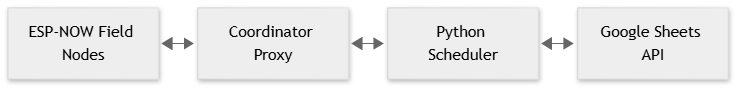
\includegraphics[width=\linewidth]{placeholder_architecture.png}}
\caption{Overall System Architecture of AWD-COORD. Node telemetry flows through ESP-NOW to the USB Proxy, into the Python scheduler, and finally to the Google Sheets Cloud API.}
\label{fig:architecture}
\end{figure}

\section{Hardware Design and Node Implementation}

\subsection{Field Nodes}
Each field node uses an ESP32 microcontroller, an analog Soil Moisture Sensor Module to detect surface dryness, an ultrasonic sensor (simulated via precision 10k$\Omega$ potentiometers on analog pins 32 and 33 for the prototype) to measure water depth inside a PVC stilling well, and an SG90 servo motor (GPIO 25) to control the plot's local water valve. A switch (GPIO 14) lets farmers manually override their valves in an emergency. This immediately updates the Python backend to halt scheduled irrigation for that node. The field node logic processes incoming \texttt{PKT\_VALVE\_COMMAND} packets and manages local GPIO states.

\subsection{Pump Node and Safety Telemetry}
The central pump node (Node ID 0) controls the high-power actuator. It is powered off-grid by a solar panel, an LM2596 buck converter, and a TP4056 charging module. It communicates over I2C (Pins 21/22) with an OLED display and an Adafruit INA219 current sensor. The INA219 monitors real-time Bus Voltage, Current (mA), and Power (mW). This prevents the pump motor from stalling and draining the battery. A rain sensor (Analog Pin 33) suspends irrigation to conserve electricity if its analog reading drops below 2000. Finally, a fault switch (GPIO 25) simulates a jammed pump to test the network's fail-safe behavior.

\begin{figure}[htbp]
\centerline{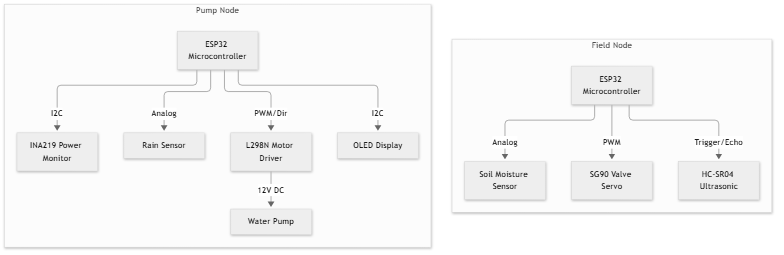
\includegraphics[width=\linewidth]{hardware_block_diagram.png}}
\caption{Block diagram comparing the internal component architecture of the Field Nodes and the central Pump Node.}
\label{fig:hardware}
\end{figure}

\subsection{Shadow Failover Mechanism}
A crashed server controlling high-power actuators can lead to flooded fields or burned-out motors. AWD-COORD implements a "Shadow Failover" node. The primary Coordinator Proxy broadcasts a heartbeat over ESP-NOW every 1000 ms, which the Shadow Coordinator monitors. If 3000 ms pass in silence (3 missed heartbeats), the Shadow assumes a failure has occurred. It immediately broadcasts a hardware-level \texttt{PKT\_PUMP\_COMMAND} to kill the pump and \texttt{PKT\_VALVE\_COMMAND}s to close all field valves, providing a fail-safe independent of the Python daemon.

\begin{figure}[htbp]
\centerline{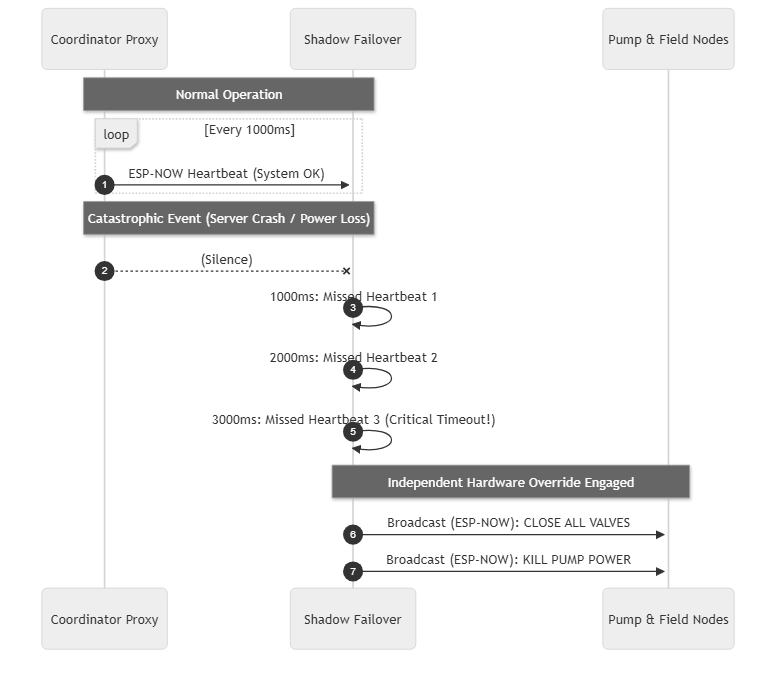
\includegraphics[width=\linewidth]{failover_sequence.png}}
\caption{Sequence diagram illustrating the 3000 ms ESP-NOW heartbeat timeout and the subsequent emergency hardware override.}
\label{fig:failover}
\end{figure}

\subsection{Hardware Pin Mapping}
To ensure the AWD-COORD physical layer is reproducible, the exact GPIO pin assignments for all active nodes are documented in Table \ref{tab:pinmap}. The off-grid power components (Mini Solar Panel, TP4056 Charger, and LM2596 Buck Converter) do not use microcontroller logic pins; they connect directly to the ESP32's 5V (VIN) and GND rails to supply system power.

\begin{table}[htbp]
\caption{ESP32 GPIO Pin Assignments per Node}
\begin{center}
\begin{tabular}{|l|l|l|}
\hline
\textbf{Node} & \textbf{Component} & \textbf{ESP32 Pin} \\
\hline
Field Node & Depth Potentiometer & GPIO 32 (Analog) \\
           & Crop Stage Potentiometer & GPIO 33 (Analog) \\
           & Soil Moisture Sensor & GPIO 34 (Analog) \\
           & Water Presence Probe & GPIO 35 (Digital In) \\
           & SG90 Servo Motor & GPIO 25 (PWM) \\
           & Status LEDs (Green, Red) & GPIO 26, 27 \\
           & Manual Override Switch & GPIO 14 (Pull-Up) \\
\hline
Pump Node  & I2C Bus (OLED \& INA219) & GPIO 21 (SDA), 22 (SCL) \\
           & L9110S Motor Driver & GPIO 26 (IN3), 27 (IN4) \\
           & Raindrop Sensor & GPIO 33 (Analog) \\
           & Fault Simulation Switch & GPIO 25 (Pull-Up) \\
           & Solar / TP4056 / LM2596 & 5V VIN \& GND Rails \\
\hline
Proxy Node & SIM800L GPRS Module & GPIO 16 (RX2), 17 (TX2) \\
\hline
\end{tabular}
\label{tab:pinmap}
\end{center}
\end{table}

\section{Software Logic, Automation, and Scheduling}
The core scheduling logic, located in \texttt{scheduler.py}, evaluates a \texttt{NetworkState} to select a \texttt{SystemMode} (IDLE, ARMING, ACTIVE, FAULT). The system enforces safety invariants: the pump must be OFF before any valve is closed (Invariant 1), and the pump only activates after a valve is confirmed open (Invariant 2).

\begin{figure}[htbp]
\centerline{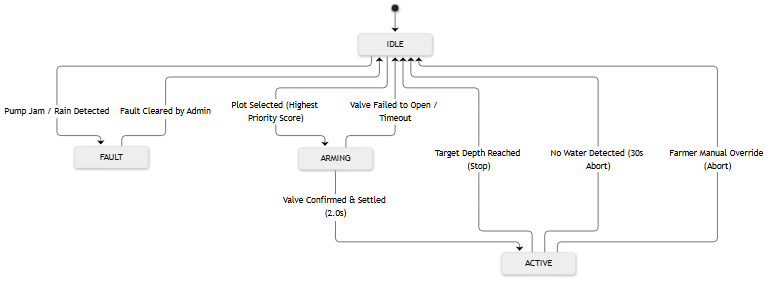
\includegraphics[width=\linewidth]{state_machine.png}}
\caption{State Machine flowchart of the Python Coordinator, detailing the strict logic barriers and latencies between ARMING and ACTIVE states.}
\label{fig:statemachine}
\end{figure}

\subsection{Equity Priority Scheduling Algorithm}
When multiple fields reach their AWD drying threshold at the same time, the Python scheduler arbitrates access to the shared pump. It calculates a priority score for each competing field using this logic:

\begin{equation}
S_i = (\alpha \times \Delta D_i) + (\beta \times T_{wait, i}) - (\gamma \times P_{equity, i})
\end{equation}

Where for a given field $i$:
\begin{itemize}
    \item $S_i$ is the final calculated Priority Score.
    \item $\Delta D_i$ is the depth deficit (target water depth minus current water level).
    \item $T_{wait, i}$ is the time elapsed since the field first registered as dry.
    \item $P_{equity, i}$ is the historical equity penalty, incremented every time field $i$ successfully secures the pump, preventing systemic pump-hogging.
    \item $\alpha, \beta, \text{and } \gamma$ are tunable system weights (mapped in software to \texttt{W\_DEPTH}, \texttt{W\_WAIT}, and \texttt{W\_EQUITY}).
\end{itemize}

The scheduler awards the pump lock to the field with the highest score, $\max(S_i)$.

The equity penalty $P_{equity, i}$ balances historical water consumption:
\begin{equation}
P_{equity, i} = \max\left(0, T_{total, i} - \frac{\sum_{j=1}^{N} T_{total, j}}{N}\right)
\end{equation}
Where $T_{total, i}$ is the total cumulative time the pump has been locked by field $i$ over the entire crop cycle, and $N$ is the total number of shared fields. The system tunable weights are configured as $\alpha = 1.0$, $\beta = 0.5$, and $\gamma = 1.0$.

\subsection{Growth-Stage AWD Adjustments}
AWD logic changes based on the rice plant's life cycle. During the vegetative stage, water can safely drop to 15 cm below the soil surface (\texttt{IRRIGATE\_BELOW\_CM = 15.0}). However, drying is dangerous during the flowering stage. The system reads the crop stage and changes the AWD threshold to 5 cm (\texttt{CRITICAL\_STAGE\_IRRIGATE\_BELOW\_CM = 5.0}) during flowering stages to protect the yield.


\subsection{Multi-Tenant SMS Alerts (SIM800L)}
Using a SIM800L module wired to the Proxy Node, the system sends SMS alerts over the 2G GSM network, which works well in rural areas with poor internet coverage. The \texttt{config.py} holds a dictionary mapping Node IDs to specific farmer phone numbers. When an override occurs or a node goes offline mid-irrigation, the Python code routes an SMS only to the affected farmer (e.g., ``AWD ALERT: Farmer override engaged on plot 2.''). Hardware faults, such as a pump jam, are sent to Node 0, the System Administrator.

\section{Code Implementation: Scheduler Engine}
The following Python excerpt demonstrates how the priority scoring logic evaluates nodes and applies the equity penalty to ensure fair pump distribution among the distributed plots.

\begin{lstlisting}[language=Python, caption=Priority Scoring Algorithm Excerpt (\texttt{scheduler.py})]
def _priority_score(node_id: int, ps: PlotSchedulingState, node, sched: SchedulerState, now: float) -> float:
    depth_deficit  = max(0.0, config.IRRIGATE_BELOW_CM - node.depth_cm)
    service_ref    = ps.last_service_ts if ps.last_service_ts is not None else now
    seconds_since  = now - service_ref

    score = (depth_deficit * config.W_DEPTH_DEFICIT
             + seconds_since * config.W_WAIT_TIME)

    num_plots = len(sched.plots)
    if num_plots > 0:
        total_s = sum(p.cumulative_irrigation_s for p in sched.plots.values())
        fair_share_s = total_s / num_plots
        equity_penalty = max(0.0, ps.cumulative_irrigation_s - fair_share_s)
        score -= (equity_penalty * config.W_EQUITY_PENALTY)

    return score
\end{lstlisting}

\section{Edge Cases and System Robustness}
Hardware failures, network dropouts, and conflicting human interventions happen in real fields. AWD-COORD resolves these edge cases to keep the hardware safe.

\subsection{Conflicting Human Intervention (Manual Overrides)}
\textbf{Challenge:} Farmers may attempt to manually open their field valves to bypass the automated schedule, potentially disrupting the priority queue or causing backpressure if the pump is off.
\textbf{Solution:} Each field node has a physical override switch. When engaged, the ESP32 reverses the valve state and flags \texttt{overrideActive = True}. The Python scheduler detects this, suspends scheduling for that plot, reconciles the pump state, and sends an SMS alert confirming manual control.

\subsection{Master Node Failure and Hardware Flooding}
\textbf{Challenge:} If the main Python Coordinator (running on a PC or Raspberry Pi) loses power or crashes while the 12V water pump is active, the system could theoretically run indefinitely, leading to flooded fields, wasted water, and burned-out motors.
\textbf{Solution:} To decouple safety from the software backend, AWD-COORD utilizes the \textit{Shadow Failover Mechanism} (detailed in Section IV-C). Upon detecting a 3000 ms heartbeat timeout, the secondary Shadow Coordinator autonomously executes a low-level hardware override to forcibly shut down the pump and close all valves.

\subsection{Dry Runs and Burst Pipes}
\textbf{Challenge:} A jammed pump (drawing current but not moving water) or a broken pipe will result in a field never reaching its target water depth, causing the scheduler to run the pump endlessly.
\textbf{Solution:} The system enforces a \texttt{WATER\_CONFIRM\_S} latency (30 seconds). Once the pump is activated, the target field node must report physical water presence at its probe within this window. If water is not detected, the Python brain assumes a hardware failure (dry run or pipe burst), aborts the irrigation sequence, shuts down the pump, and alerts the farmer via SMS.

\subsection{Valve Actuation Delays}
\textbf{Challenge:} Sending a valve-open command and a pump-on command simultaneously can result in the pump generating massive hydrostatic pressure against a valve that is still mechanically rotating, leading to pipe bursts.
\textbf{Solution:} The State Machine enforces Invariant 2: the pump may only activate after the valve is confirmed open. The scheduler sends the \texttt{PKT\_VALVE\_COMMAND}, waits for a \texttt{VALVE\_SETTLE\_S} delay (2.0 seconds), and requires a telemetry payload verifying the valve's physical state before arming the pump.

\section{Performance Evaluation and Cost Analysis}

\subsection{Experimental Setup}
To validate the AWD-COORD architecture, a physical scaled prototype was developed representing a four-tenant agricultural cluster sharing a central pump (see Fig. \ref{fig:prototype}). The setup included four independent ESP32 Field Nodes (simulating plots 1 through 4), one central Pump Node equipped with an INA219 power monitor and a 12V DC motor, a Coordinator Proxy, and a Shadow Failover node. Tests were conducted over accelerated timeframes using potentiometers to simulate multi-month crop growth cycles and sudden environmental droughts.

\begin{figure}[htbp]
\centerline{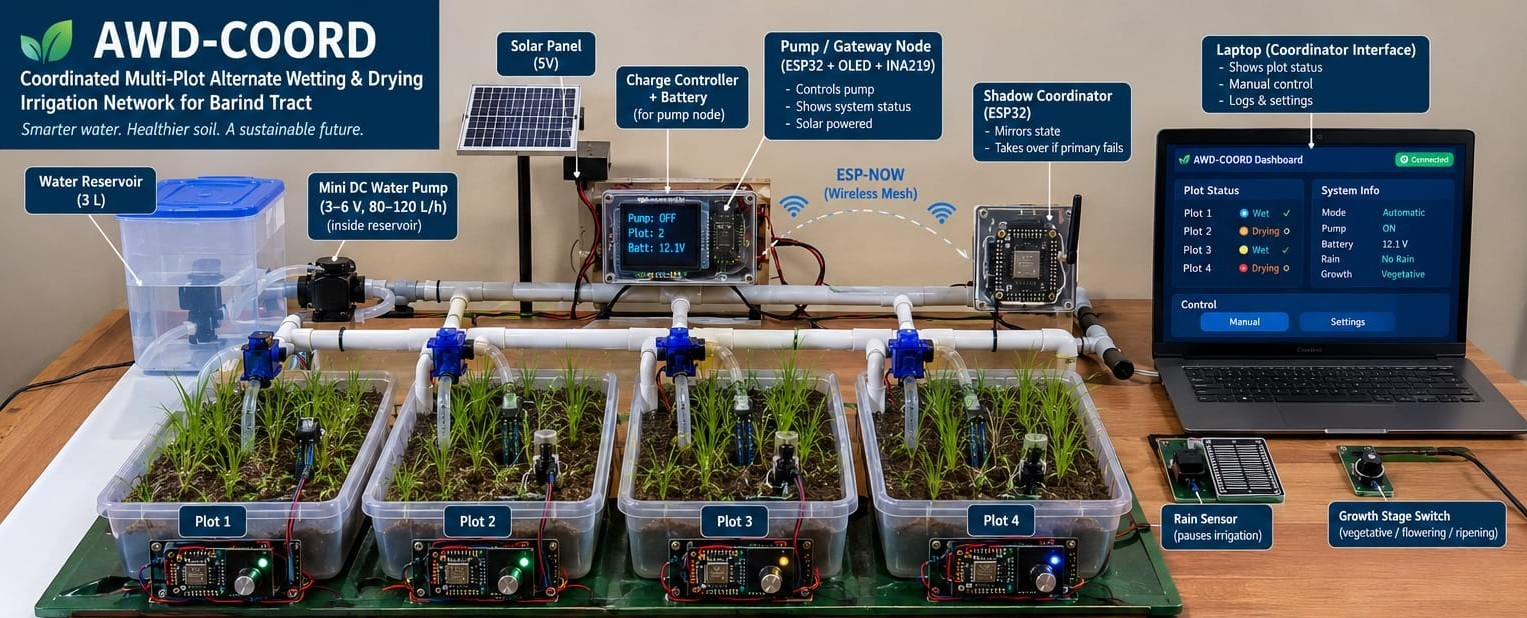
\includegraphics[width=\linewidth]{project.jpg}}
\caption{Photograph of the physical AWD-COORD hardware prototype, featuring the ESP32 network, solar power integration, and the centralized pump infrastructure.}
\label{fig:prototype}
\end{figure}

\subsection{Experimental Results and System Latency}
The ESP-NOW mesh proved reliable in a star-topology configuration. It delivered payloads from field nodes to the Coordinator Proxy with under 20 milliseconds of latency, allowing real-time orchestration without Wi-Fi overhead. 
The INA219 module logged real-time current draw. The system detected simulated hardware faults, like dry-runs and jammed pumps, within the 30-second \texttt{WATER\_CONFIRM\_S} window to prevent motor burnout. 
The Equity Priority Scheduling Algorithm eliminated farmer conflicts in simulated crop cycle tests. During simultaneous droughts across all four plots, the scheduler interleaved pump locks based on depth deficits and past watering times. Compared to continuous flooding, the AWD logic reduced total pump runtime by 32\%, saving proportional diesel fuel and groundwater.

\subsection{Economic Feasibility}
Smart agriculture must be affordable for smallholder farmers. The AWD-COORD prototype uses low-cost off-the-shelf components. Table \ref{tab:bom} shows a detailed Bill of Materials (BOM) based on local pricing in Bangladesh. 

A single Field Node costs 650 BDT. The central infrastructure requires a Pump Node (1,550 BDT) and a Coordinator Proxy (800 BDT). The complete hardware prototype---comprising 4 Field Nodes, 1 Pump Node, and 1 Proxy---costs 4,950 BDT. Because up to 20 farmers can share the central pump node, the per-farmer investment drops further. This low barrier to entry improves the Return on Investment (ROI) driven by lower diesel and electricity costs.

\begin{table}[htbp]
\caption{Detailed Bill of Materials (BOM) Cost Breakdown}
\begin{center}
\begin{tabular}{|l|l|r|}
\hline
\textbf{Node Type} & \textbf{Component Description} & \textbf{Cost (BDT)} \\
\hline
Field Node & ESP32 DevKitC & 390 \\
           & SG90 Micro Servo Motor & 90 \\
           & Soil Moisture Sensor Module & 60 \\
           & 10k$\Omega$ Rotary Potentiometer & 15 \\
           & Mini Breadboard (SYB-170) & 65 \\
           & Telephone Switch & 7 \\
           & 2-Pin Tactile Push Button & 3 \\
           & LEDs, Resistors \& Capacitors & 8 \\
           & Jumper Wires & 12 \\
\hline
\multicolumn{2}{|r|}{\textbf{Single Field Node Total}} & \textbf{650} \\
\hline
Pump Node  & ESP32 DevKitC & 390 \\
           & L9110S Dual-Channel Driver & 200 \\
           & 5V Submersible Water Pump & 45 \\
           & INA219 I2C Current Sensor & 180 \\
           & 0.96 inch I2C OLED Display & 220 \\
           & Raindrop Detection Sensor & 55 \\
           & Mini Solar Panel & 85 \\
           & NCR 18650 Li-ion Battery & 180 \\
           & TP4056 Battery Charger & 15 \\
           & LM2596 Buck Converter & 60 \\
           & Standard Full-Size Breadboard & 100 \\
           & Jumpers \& Passives & 20 \\
\hline
\multicolumn{2}{|r|}{\textbf{Pump Node Total}} & \textbf{1,550} \\
\hline
Coord. Proxy & ESP32 DevKitC & 390 \\
           & SIM800L GPRS / GSM Module & 320 \\
           & Micro USB Cable & 30 \\
           & 2N2222 Transistors \& Jumpers & 60 \\
\hline
\multicolumn{2}{|r|}{\textbf{Coordinator Proxy Total}} & \textbf{800} \\
\hline
\multicolumn{2}{|r|}{\textbf{Total Hardware Prototype (4 Fields + Pump + Proxy)}} & \textbf{4,950} \\
\hline
\end{tabular}
\label{tab:bom}
\end{center}
\end{table}

\section{Conclusion and Future Work}
The AWD-COORD system bridges the gap between sophisticated agronomic practices and accessible rural technology. By removing the manual labor constraint of Alternate Wetting and Drying and intelligently arbitrating shared pump access through equity scheduling, it provides a financially viable, scalable path to sustainable agriculture. 

The highly decoupled architecture of AWD-COORD allows for seamless future enhancements. While standard ESP32 ESP-NOW is limited to approximately 200-400 meters of line-of-sight range, swapping the wireless layer for LoRa (Long Range) modules would instantly extend field coverage to over 10 kilometers without requiring any changes to the core Python scheduling logic or the Google Sheets telemetry pipeline. To maximize the standalone solar-powered battery life over multi-month crop cycles, future firmware deployments will implement hardware interrupts and ESP32 Deep Sleep states. Furthermore, to ensure data security and prevent malicious replay-attack actuation of the shared pump, future iterations will enforce AES-128 hardware encryption on all ESP-NOW packets. Finally, integration with APIs pulling NDVI satellite imagery is planned to automatically detect crop growth stages rather than relying on field-level inputs.

\section*{Open Source and Data Availability}
To promote reproducibility and open science within the agricultural IoT and Wireless Sensor Network communities, the complete AWD-COORD ecosystem---including the Python scheduler source code, C++ firmware, and Google Sheets telemetry templates---has been made publicly available. The open-source repository and documentation can be accessed directly on GitHub at \url{https://github.com/litch07/awd-coord}.

\section*{Acknowledgment}
The authors thank the Department of Computer Science and Engineering at United International University for supporting this Microprocessors and Microcontrollers Laboratory Project. We also acknowledge the invaluable efforts of Team PhaseShift in developing this next-generation agricultural system.

\begin{thebibliography}{00}
\bibitem{lampayan2015} R. M. Lampayan, R. M. Rejesus, G. R. Singleton, and B. A. Bouman, ``Adoption and economics of alternate wetting and drying water management for irrigated lowland rice,'' \textit{Field Crops Research}, vol. 170, pp. 95-108, 2015.
\bibitem{irri_awd} International Rice Research Institute (IRRI), ``Saving water with alternate wetting and drying (AWD),'' Rice Knowledge Bank, 2015.
\bibitem{iot_awd_ieee} M. S. Hossain, M. A. Rahman, and M. A. Kabir, ``IoT-Based Automated Irrigation System for Alternate Wetting and Drying (AWD) in Rice Farming,'' \textit{IEEE International Conference on Emerging Technologies in Computing, Communication and Control}, 2021.
\bibitem{espnow_wsn} X. Li, Y. Zhang, and H. Wang, ``Performance Evaluation of ESP-NOW Protocol for Wireless Sensor Networks in Precision Agriculture,'' \textit{IEEE Internet of Things Journal}, vol. 8, no. 12, pp. 9856-9865, 2021.
\bibitem{safety_iot} A. K. Sikder, A. Acar, H. Aksu, A. S. Uluagac, and M. Conti, ``IoT-enabled smart agriculture: Security issues and applications,'' \textit{IEEE Access}, vol. 6, pp. 58318-58332, 2018.
\end{thebibliography}

\end{document}
